\chapter{Umsetzung}
Mit der Umsetzung des Konzeptes zeigt sich wie gut dieses Gelungen ist. Nachdem nun geklärt ist, wie die Anwendung aussehen soll und welche Werkzeuge verwendet werden, muss eine Testumgebung aufgebaut werden. Ebenfalls muss der Umgang mit den Frameworks und der \ac{IDE}, zu deutsch integrierte Entwicklungsumgebung, vertraut sein.

\section{Aufbau einer Testumgebung}
\label{sec:integration_ace}
Der Server im Smarthome Lab erledigt rund um die Uhr aufgaben. Dabei überwacht er den Zustand verschiedener Geräte und sorgt dafür das diese erreichbar sind. Auf ihm liegen auch Medien und der Webauftritt, welcher über einen Webserver läuft. Dies muss immer zuverlässig funktionieren. Damit der Betrieb nicht eingeschränkt ist, muss eine virtuelle Testumgebung geschaffen werden. Für diesen Zweck wurde ein Abbild des Servers erzeugt, als alles zuverlässig gearbeitet hat. Auf dem Abbild war neben dem Betriebssystem auch der Webserver mit Webauftritt und die MySQL-Datenbank zu finden. Da diese identisch mit den Daten des Servers waren, konnte realistisch getestet werden. Durch das einfache erstellen von Sicherheitskopien konnte risikofrei Software installiert werden um zu schauen, wie sich diese auf das System auswirkt. Mit den verschieden Sicherheitskopien, konnte bei Problemen immer auf einen alten Stand zurückgegriffen werden.


\begin{figure}[bh]
	\centering
	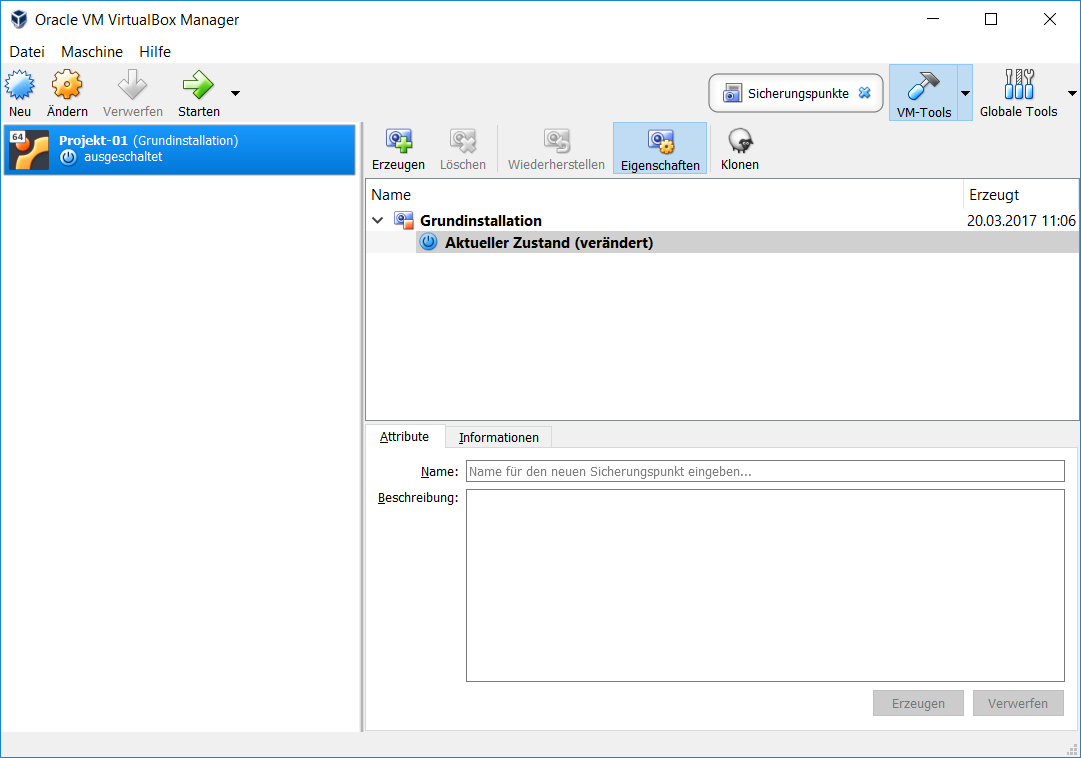
\includegraphics[scale=0.4]{content/pictures/vmware.png}
	% bosch_iot_poll.png: 0x0 pixel, 300dpi, 0.00x0.00 cm, bb=
	\caption{VM-Ware mit geladenem Abbild}
	\label{fig:vmware}
\end{figure}

 In Abbildung \ref{fig:vmware} sieht man den VM-Ware Player. Dieser ist ein kostenloses Tool um Virtuelle Maschinen abzuspielen. Der VM-Ware Player simuliert dabei Hardware, welche im Live-betrieb verändert werden kann. \autocite{vmwareinc.2018} In diesem Fall wird der Server aus dem Smarthome Lab nur Simuliert. Dabei kann ihm mehr speicher hinzugefügt werden, oder auch Seicher entfernt werden. So kam es zu dem Problem, das auf der \ac{VM} nicht ausreichen Festplattenspeicher zur Verfügung stand. In diesem Fall musste die komplette \ac{VM} vergrößert werden. Dies ist mit VM-Ware Player nicht machbar. Unter Windows wird bei der Installation von VM-Ware Player auch der Vdiskmanager installiert. Ein Werkzeug, welches sich über die Kommandozeile steuern lässt. So lässt sich mit dem Befehl \textit{vmware-vdiskmanager -x 100Gb vm.vmdk}, im Verzeichnis der \ac{VM}, die Größe verändern. \autocite{ThomasKrennAG.2018} Damit war ein Vergrößern der \ac{VM} zwar möglich, der zusätzliche Speicher stand zwar physisch, durch eine größere \ac{VM} Datei zur Verfügung, konnte jedoch nicht verwendet werden. In der \ac{VM} wurde ein sogenannter Snapshot verwendet. Bei einem Snapshot, handelt es sich um eine Kopie der \ac{VM} zu einem bestimmten Zeitpunkt. Dieser musste ebenfalls vergrößert werden. Da die Quellen hierzu rar waren, erforderte die Lösung eine lange Suche. Die Lösung ist, mit dem Vdiskmanager den Snapshot auf die gleiche Größe zu bringen. Der Speicher wird nun angezeigt, kann jedoch noch nicht Verwendet werden, da er keiner Partition zugewiesen worden ist. Dies ist über das Betriebssystem, Ubuntu Server 16.04, welches auf der \ac{VM} läuft nicht einfach zu bewerkstelligen. Eine Lösung ist es Ubuntu 18.04 zu verwenden. Dabei wir ein Abbild der DVD, welche für die Installation von Ubuntu benötig wird, in das Virtuelle DVD Laufwerk gelegt. Ubuntu kann ohne Installation verwendet werden. Es liefert das Programm GPartet, mit welchem sich der neue, noch nicht zugewiesene Speicher, der Serverpartition zuweisen lässt. Mit einem Neustart der \ac{VM} und dem Entfernen des Images aus dem virtuellen Laufwerk, hat die \ac{VM} nun ausreichend Festplattenkapazität.\autocite{automatix.}

\subsection{Integration in das Netzwerk}
Da es sich bei der \ac{VM} um ein direktes Abbild des Servers im Smarthome Lab ist, hat es auch die identischen Eigenschaften. So auch die \ac{MAC}. Mit der \ac{MAC}-Adresse soll der Netzwerkkarte eine eindeutige Identifikationsnummer zugewiesen werden. Dies geschieht schon bei der Herstellung und der Router kann damit Geräte identifizieren, welche im Netzwerk eingebunden sind. Damit ist dem Router bewusst welches Gerät, welche Pakete und welche \ac{IP} erhält. \autocite{Zisler.2016} Solche \acp{IP} sollen weltweit eindeutig sein, sind es aber nicht, wenn es nicht gewünscht ist. Bei einem Abbild erwartet der User ein identisches System. Möchte er dieses System allerdings im gleichen Netzwerk einsetzen, so wird der Router die Pakte an Router und an die \ac{VM} senden, da der Router nicht unterscheiden kann, wer der Korrekte Empfänger ist. Wird das nicht korrigiert, kann es leicht passieren das unerwünschte Änderungen am Server und nicht an der \ac{VM} unternommen werden. Denn die \ac{VM}, wie auch der Server werden über \ac{SSH} angesteuert. Dabei wird ein Programm verwendet, in diesem Fall Putty, welches eine sichere Verbindung über das Netzwerk zum Server oder zur \ac{VM} aufbaut. Ist man nun im Netzwerk des \ac{SHL} ist nicht klar ob die \ac{VM} oder der Server angesprochen wird. Denn schließlich haben beide die selbe \ac{IP} zugewiesen bekommen. Eine Lösung für dieses Problem wird direkt in vmware-Player zur Verfügung gestellt. In Abbildung \ref{fig:vmwaremac} sieht man das man die \acl{MAC} einfach in einem Textfeld anpassen kann. Mit einer neuen \acl{MAC} unterscheidet das Netzwerk nun beide \textit{Netzwerkkarten}. Damit erhält die \acl{VM} nun eine neue \ac{IP} und ist damit eindeutig adressierbar.

\begin{figure}[bh]
	\centering
	
	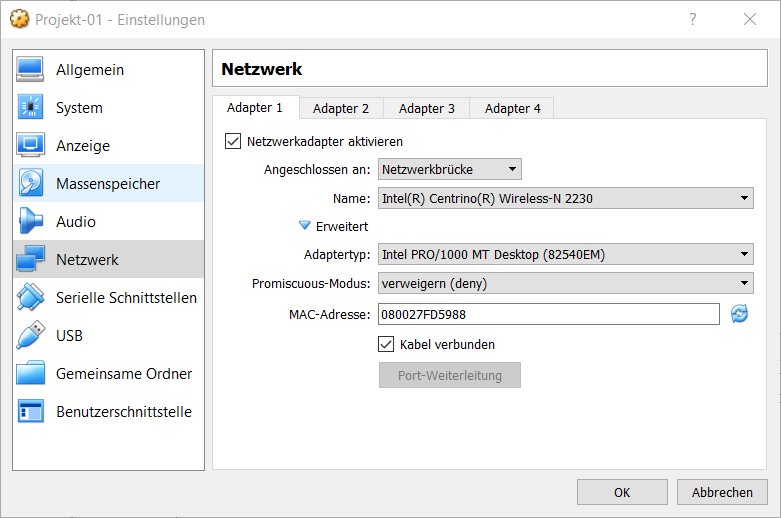
\includegraphics[scale=0.6]{content/pictures/macadresse.png}
	% bosch_iot_poll.png: 0x0 pixel, 300dpi, 0.00x0.00 cm, bb=
	\caption{ Netzwerkeigenschaften im  VM-Ware-Player}
	\label{fig:vmwaremac}
\end{figure}


\subsection{MySQL}
Auf dem Server stand bereits eine MySQL Datenbank zur Verfügung.  Es handelt sich hierbei um eine relationale Datenbank. \autocite{Oracle.} MySQL steht unter der \ac{GPL} 2.0 und ist OpenSource. WordPress setzt eine MySQL oder eine MariaDB voraus.\autocite{akbarali} Die Daten der Tabellen, welche Wordpress genutzt hatte, waren alle weiter erreichbar und konnten verwaltet werden. Die Daten für die Datenbank selbst haben gefehlt. Wenn diese Daten fehlen, so ist es möglich die Datenbank, mit Adminrechte, ohne Passwort zu starten. Nach einem solchen Start, kann das Passwort beliebig verändert werden. In diesem Fall wurde auch das von der Datenbank untersagt. Eine Datenbank war für die kommende Arbeit notwendig und somit auch der Zugriff. Da dies nicht möglich war, musste die Datenbank neu installiert werden. Für diesen Zweck wurden alle Tabellen und Datensätze in eine Datei gesichert. Über ein Plugin, welches in WordPress installiert wurde, konnte eine solche Datei erzeugen. Mit der Neuinstallation der MySQL-Datenbank wurde ein bekanntes Passwort vergeben. Die Daten wurden importiert und es mussten nur noch wenige Daten angepasst werden, da es sich um die identischen Daten handelte. 

\subsection{Nginx}
Vorinstalliert war auch der WebServer Nginx. Standardmäßig handelt es sich hier um einen Webserver, wellcher HTTP anfragen entgegennimmt und und GET Anfragen verarbeitet. Um einen WordPress Blog welcher \ac{PHP}, JavaScript und \ac{HTML} benötigt, ist das völlig ausreichen.\autocite{akbarali} Für weitere Verarbeitungen wie POST, PUT und DELETE müssen diverse Konfigurationen an Nginx vorgenommen werden.\autocite{MFB.2013}

\section{XAMPP}
Um lokal die Webanwendung entwickeln zu können, ist es nötig auf der lokalen Maschine MySQL und \ac{PHP} installiert zu haben. Eine Lösung, welche für dieses Problem angeboten wird, ist XAMPP. Es handelt sich um eine frei Paketsammlung zu welcher auch \ac{PHP} und MySQL gehören und wurde von den Apache Friends entwickelt.\autocite{ApacheFriends.} Es steht unter der \ac{GPL}. Durch seine \ac{UI} ist das starten von \ac{PHP} oder MySQL mit einem klick erledigt. Sollte eine Datenbankabfrage mal nicht möglich sein, könnte eine Fehlerquelle sein, das der MySQL-Server nicht läuft. 

\newpage
\section{Austausch von Daten}
Für einen sicheren Datentransfäre von der Entwicklungsmaschine zur \acl{VM} wird \ac{SCP} verwendet. Um dies nicht über ein \ac{CLI} machen zu müssen, gibt es software mit einer grafischen Oberfläche. Mit solch einer Software wird eine sichere Verbindung aufgebaut. Ein Datentransfäre funktioniert so ähnlich wie bei einem \ac{FTP} Tool. Man zieht die zu übertragenen Dateien mit der Maus in das Zielverzeichnis. Ein solcher Vertreter ist, unter dem Betriebssystem Windows, WinSCP, welches in Abbildung \ref{fig:winscp} zu sehen ist.

\begin{figure}[bh]
	\centering
	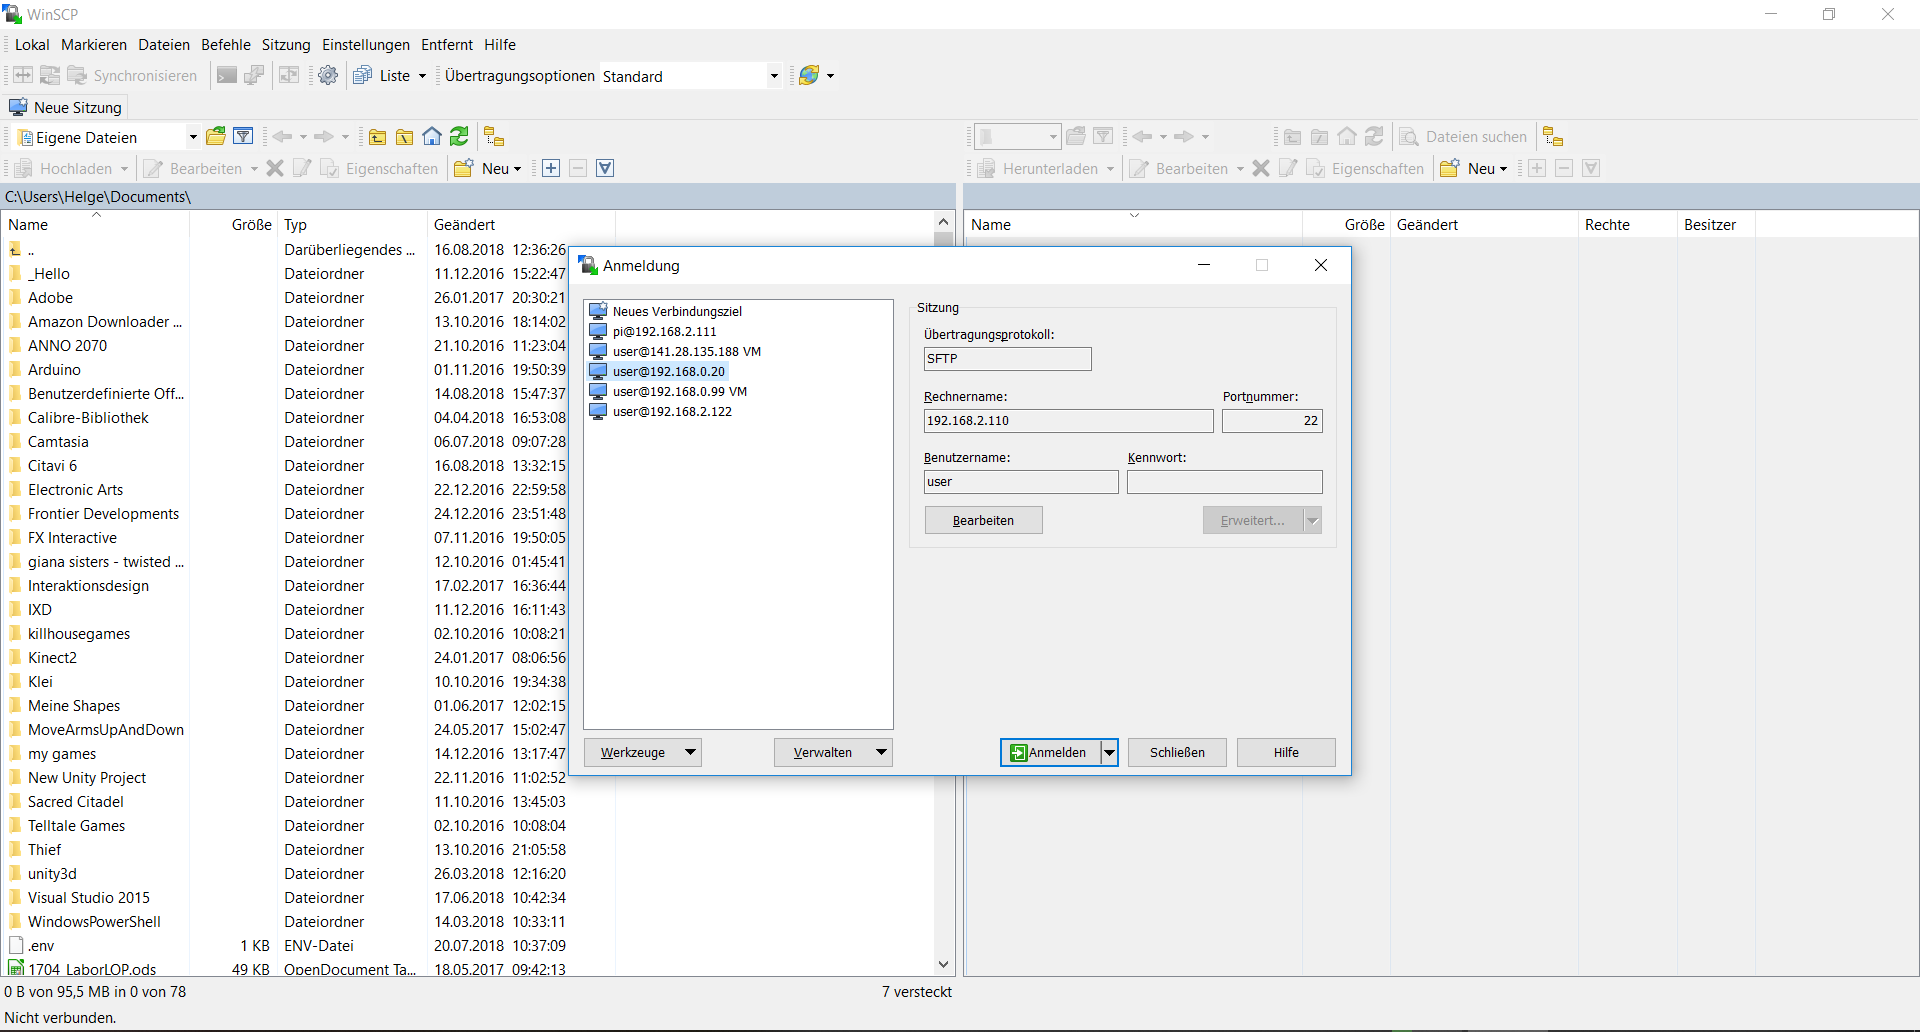
\includegraphics[scale=0.3]{content/pictures/winscp.png}
	% bosch_iot_poll.png: 0x0 pixel, 300dpi, 0.00x0.00 cm, bb=
	\caption{ WinSCP}
	\label{fig:winscp}
\end{figure}



\section{Frontend}
\label{chapter:frontend}
Bei einem Frontend spricht man von dem was der Anwender sieht. Es handelt sich um Buttons, Links, Farben, Layouts \ac{uvm.}. Wie in Kapitel \ref{chapter:frameworkchoice} erwähnt, wurde Angular für die Umsetzung des Frontends verwendet. Zum Entwicklungszeitpunkt befand sich Angular in der Version 5, was sich im Laufe der Umsetzung geändert hat. Dies nahm jedoch keinen Einfluss auf die Entwicklung und die Webanwendung wurde mit Angular 5 fertig entwickelt. Es erfüllt die Aufgaben einer Komponenten basierten Darstellung von verschiedenen Bausteinen.  Durch seine Feste Struktur von Services, Components (\ac{z. Dt.} Komponenten) und Views (\ac{z. Dt.} Ansichten) \autocite{Clow.2018}, ist es übersichtlich und Kenntnisse mit Angular reichen, um sich einzuarbeiten. Es wird von Google entwickelt, aber profitiert von einer sehr aktiven Community (\ac{z. Dt.} Gemeinschaft). Diese Entwickelt Module, welche den Funktionsumfang von Angular erweitern. Dies ermöglicht die \ac{MIT}-Lizens, welche den Code frei einsehbar macht und erlaubt diesen zu verändern.\autocite{BonnyKern.2017}

\subsection{Installation von Angular}
Bevor man Angular installieren kann, muss erst einmal Node.js auf dem Entwicklersystem installiert werden. Es ist für die gängigen Betriebssysteme wie Windows, MacOS und Linux verfügbar. Es wird kostenfrei auf \url{https://nodejs.org/de/} Angeboten. Bei Node.js handelt es sich um eine Laufzeitumgebung. \autocite{Node.js.2018} Dies ist vergleichbar mit Java, welches für die Entwicklung von Programmen benötigt wird, welche in Java geschrieben sind. Im Fall von Node.js wird JavaScript \ac{bzw.} EcmaScript verwendet. Mit der Installation von Node.js wird auch der \ac{NPM} installiert. Bei \ac{NPM} handelt es sich um ein Tool mit welchem Programme, Frameworks \ac{uvm.} installiert werden können. Die Angebotenen Dienste und Programme werden auf \url{https://www.npmjs.com} angeboten. Auch Angular wird hier angeboten und damit auch unzählige Erweiterungen für Angular. Möchte man Angular nun installieren geschieht das über das \acl{CLI}. Hier bei kann mittels Parameter entschieden werden ob etwas für das ganze Betriebssystem global oder nur lokal für ein einzelnes Projekt installiert werden soll. Im falle von Angular geschieht das global. Der Befehl zum installieren findet man ebenfalls auf \url{https://www.npmjs.com}. Werden keine weiteren Parameter angegeben, wird immer die neuste Version heruntergeladen.

\begin{lstlisting}[language=sh, frame=single]
$  npm install angular -g
\end{lstlisting} 

\subsection{Commandlineinterface von Angular}
Angular selbst liefert seit der Version 2 ein \acl{CLI} mit. Mit diesem \ac{CLI} ist es möglich Angular Projekte zu verwalten. Mit einer Zeile kann ein komplettes Projektsetup erzeugt werden. Mit Hilfe von Parameter kann angegeben werden, wie Anwendung gestylet wird. Dabei kann man beispielsweise wählen ob man die Anwendung mit \ac{CSS} oder mit \ac{SASS} gestalten möchte. Bei \ac{SASS} handelt es fast um die gleiche Syntax wie \ac{CSS}. Es unterscheidet sich in dem Punkt, das es möglich ist Blöcke zu verschachteln und es gibt die Möglichkeit Variablen zu verwenden. Da noch kein Browser nativ \ac{SASS} unterstützt, wird der \ac{SASS}-Code in \ac{CSS}-Code übersetzt. Angular wird über die Konsole verwendet indem ng angeführt wird. Im folgenden wird ein Beispielprojekt angelegt, welches zum Gestalten \ac{SASS} verwendet. Und um nicht mit anderen \ac{HTML}-Tags oder Direktiven zu kollidieren, wird jeder Anwendung für ihre eigenen Tags, was im Kapitel \ref{cha:components} erläutert wird, ein Prefix angelegt. Im Beispiel ist es bsp.


\begin{lstlisting}[language=sh, frame=single]
$  ng new Beipsielprojekt --style=sass --prefix=bsp
\end{lstlisting} 


\begin{figure}[H]
	\centering
	
	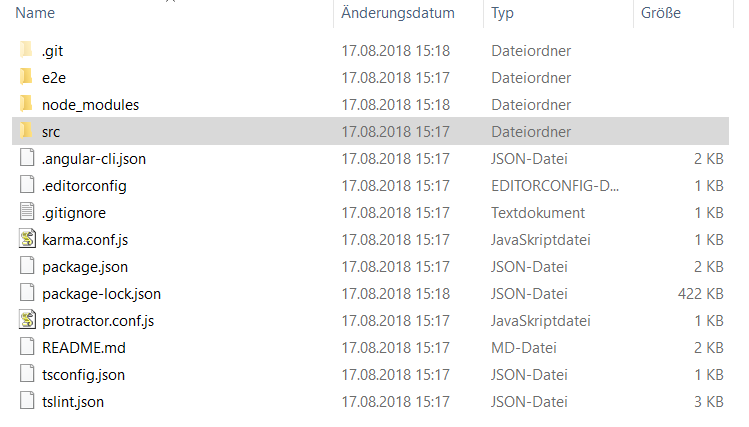
\includegraphics[scale=0.9]{content/pictures/projektordner.png}
	% bosch_iot_poll.png: 0x0 pixel, 300dpi, 0.00x0.00 cm, bb=
	\caption{ Projektordner: Angularprojekt}
	\label{fig:projektfolder}
\end{figure}

\begin{figure}[H]
	\centering
	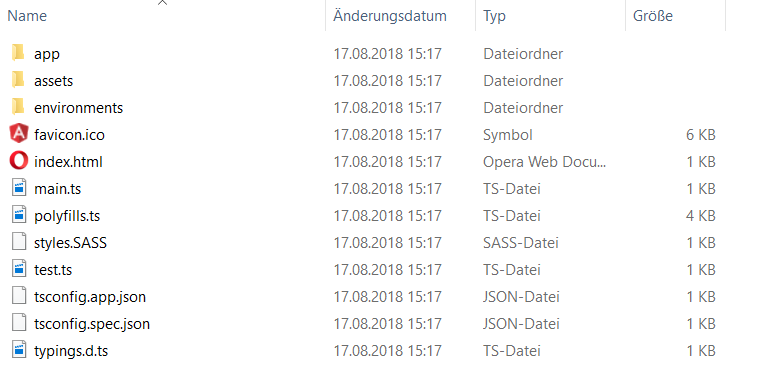
\includegraphics[scale=0.9]{content/pictures/srcfolder.png}
	% bosch_iot_poll.png: 0x0 pixel, 300dpi, 0.00x0.00 cm, bb=
	\caption{ Sourceordner in Angular Projekt}
	\label{fig:scrfolder}
\end{figure}

\begin{figure}[H]
	\centering
	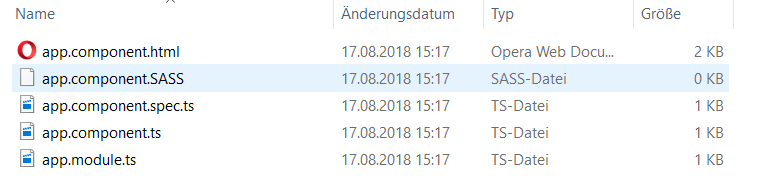
\includegraphics[scale=0.9]{content/pictures/appfolder.png}
	% bosch_iot_poll.png: 0x0 pixel, 300dpi, 0.00x0.00 cm, bb=
	\caption{ App Ordner in Src-Ordner des Angularprojektes}
	\label{fig:appfolder}
\end{figure}


Wie man in Abbildung \ref{fig:projektfolder} sehen kann wird nicht nur ein Projektsetup angelegt, sondern auch ein Ordner, in dem alle \ac{NPM} Abhängigkeiten verwaltet werden und es wird auch eine Versionverwaltung mit der Hilfe von Git übernommen, sofern Git auf dem System installiert ist. Es muss nur ein Repository angelegt und mit dem Projekt verbunden werden.




\subsection{TypeScript}
Angular selbst ist TypeScript-basiert. Das bedeutet das Angular nicht direkt JavaScript verwendet, wie es noch in Angular.js gemacht worden ist, sondern es verwendet eine Art objektorientiertes JavaScript. Bei \ac{Ecma} handelt es sich um eine Private Organisation, welche Programmiersprachen standardisiert. So handelt es sich bei JavaScript, wie es heute geläufig ist und von den meisten Browser unterstützt wird, eigentlich um EcmaScript 5. Seit wenigen Jahren existiert EcmaScript 6. Dies ist sozusagen ein JavaScript welches Klassen, Interfaces, Arrow-Functions \ac{uvm.} anbietet. Diese Features werden von vielen Entwickler gerne gesehen und lösen Probleme, mit welchen man schon länger zu tun hat und sie nur auf komplizierten Wegen lösen konnte. Allerdings unterstützen die meisten Browser noch nicht oder nur in Teilen den EcmaScript 6 Standard. An dieser stelle kommt TypeScript zum Einsatz. Eine Installation von TypeScript läuft, wie bei Angular, über \ac{NPM}. Man kann nun alle Features von EcmaScript 6 verwenden und in eine TypeScript-Datei schreiben. TypeScript übersetzt diesen Code in eine EcmaScript 5 Datei, mit welcher jeder gängige Browser umgehen kann.

Eines der größten Probleme, welche mit EcmaScript 6 gelöst wurde, ist das Problem mit this. Wenn ein Entwickler von einer anderen Objektorientierten Sprache zu JavaScript wechselt, kann er schnell verwirrt sein. In den meisten Programmiersprachen, entspricht das Schlüsselwort \textit{this}, dem Objekt der Klasse, welche man gerade schreibt. So muss das nicht in JavaScript sein und kann daher schnell zu langen Fehlersuchen führen, wenn dieses Problem nicht bewusst ist. In der Programmiersprache JavaScript ist this in der Regel, das was vor einem Punkt einer Variablen steht. Meistens handelt es sich um das Objekt. Nun ist es aber so, das man sehr häufig mit dem Window-Objekt von JavaScript arbeitet, ohne dies zu wissen. Denn die variable \textit{window} kann einer function, welche nicht neu entwickelt wurde, voran gestellt werden, muss es aber sehr häufig nicht. Ein bekanntest Beispiel ist die Funktion \textit{setTimeout()}. \textit{window.setTimeout()} ist equivalent zu \textit{setTimeout()}. Der setTimeout-Funktion muss eine Funktion als Parameter mitgegeben werden. Wird hier this verwndet, so handelt es sich um das window-Objekt. Daher kann es passieren, das der Entwickler überzeugt ist eine Variable definiert zu haben, die Konsole ihn aber auf das Gegenteil hinweist. Dies ist ein Problem das schon sehr lange existiert und auf die verschiedensten Wege gelöst wurde. Da alte Programme, welche in JavaScript programmiert wurden, weiter Funktionieren müssen, darf mit einer neuen JavaScript Version die Funktionalität von this nicht geändert werden. Deshalb wurde eine neue Möglichkeit eingeführt, mit welcher Funktionen definiert werden können. Dabei handelt es sich um die Arrow-Function. Der Name wurde gewählt weil sie statt dem Schlüsselwort function einen Pfeil verwendet. Wenn man über diese Syntax eine Funktion entwickelt und \textit{this} verwendet, so handelt es sich um das this aus der Klasse und nicht um das window-Objekt. Im folgenden, sieht man ein Beispiel für eine solche Funktion.

\begin{lstlisting}[language=sh, frame=single]
() => {
	console.log(this.firstname)
}
\end{lstlisting} 



\subsection{Module}
Mit der Verwendung von Angular, ist ein Kontakt mit Modulen nicht zu Vermeiden. Bei einem Modul wird eine komplette Angularanwendung umfasst. Dazu gehören Components, Services und Direktiven. Welche in den folgenden Kapitel erläutert werden. Module können allerdings auch nur als Funktionserweiterungen entwickelt werden.\autocite{Clow.2018} Das Framework macht es leicht, fremde Module einzubinden. Wichtige Module werden schon von dem Framework selbst angeboten. So übernehmen diese die Netzwerkkommunikation, Formularbehandlung oder auch das Darstellen von Daten. 



\subsection{Components}
\label{cha:components}
Component \ac{z. Dt.} Komponenten, sind wie der Name schon verrät Teilbereiche einer Angular-Anwendung. Bei Components handelt sich sich, im eigentlichen Sinne, um Module. Da Components aber von sehr großer Bedeutung sind verdienen Sie ihr eigenen Abschnitt und werden in den meisten Fachbücher als eigenes Kapitel behandelt. Sie werden für die Darstellung von bestimmten Teilen Verwendet. So kann eine Component sich nur um die Ausgabe einer Tabelle zuständig sein. Dabei steht diese Component für sich alleine und ist nicht von anderen Components abhängig und beeinflusst auch nicht andere Components, wenn dieses Verhalten nicht erwünscht ist. Eine Component kann in einer fremden Component verwendet werden. Ein Verschachteln von Components ist möglich. Und auch hier stehen Sie für sich. Selbst ein gestalten in \ac{CSS} ist für jede Component separat möglich. Die Ausgabe wird in \ac{HTML} geschrieben und mit TypeScript-Code erweitert.\autocite{Clow.2018}

Das \ac{CLI} von Angular unterstützt bei der Erstellung von Components den Entwickler sehr. So ist es völlig ausreichen, wenn der Benutzer beim erstellen nur die Component benennt. Angular wird für sie völlig automatisiert einen eigenen Ordner, mit \ac{CSS} bzw. \ac{SASS} Datei, einer \ac{HTML} Datei für die Darstellung, einer Testdatei und eine TypScript Datei an. Dabei werden die Dateien mit Beispielcode gefüllt und sind sofort verwendbar. Angular hällt sich an Namenskonventionen. So erhält jede Component das Wort Component in der Camel-Case Syntax, in welcher verschiedene Wörter in einer Variablen durch Großbuchstaben getrennt werden, als Suffix. Ist dies nicht erwünscht, lässt sich das durch Optionale angaben in der Konsole verhindern.

\begin{lstlisting}[language=sh, frame=single]
$  ng genarate component Beispiel
\end{lstlisting} 

\begin{lstlisting}[language=sh, frame=single]
$  ng g c Beispiel
\end{lstlisting}

In beiden Konsolenbefehle wird das Selbe ausgeführt. Die Zweite Zeile ist eine Kurzschreibweise. Das Ergebnis wird unter anderem eine Klasse mit dem Name BeispielComponent sein. 

\begin{figure}[H]
	\centering
	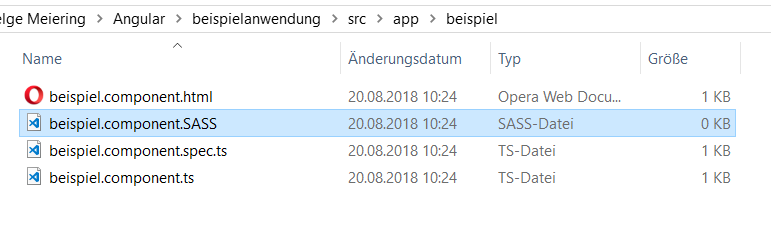
\includegraphics[scale=0.9]{content/pictures/componentfolder.png}
	% bosch_iot_poll.png: 0x0 pixel, 300dpi, 0.00x0.00 cm, bb=
	\caption{ Dateien einer Component}
	\label{fig:component}
\end{figure}

\subsection{Services}
Services lassen sich mit Controller aus dem \ac{MVC} Entwurfsmuster vergleichen. Ihre Aufgaben sind es Funktionen für Components oder anderen Services zur Verfügung zu stellen. In ihnen wird berechnet, analysiert oder auch verwaltet. Funktionen werden häufig genutzte Aufgaben Zentralisiert und müssen dadurch nur an einer einzigen Stelle angepasst werden, wenn es nötig wird. Die Ausgabe und die Darstellung wird in den Components Programmiert. \autocite{Clow.2018}

\begin{lstlisting}[language=sh, frame=single]
$  ng genarate service Beispiel
\end{lstlisting} 

\begin{lstlisting}[language=sh, frame=single]
$  ng g s Beispiel
\end{lstlisting}

Auch bei den Services wird beim Erstellen alles nötige generiert und die Camel-Case-Syntax kommt zum Einsatz. In diesem Fall würde der Service BeispielService heißen.

\begin{figure}[H]
	\centering
	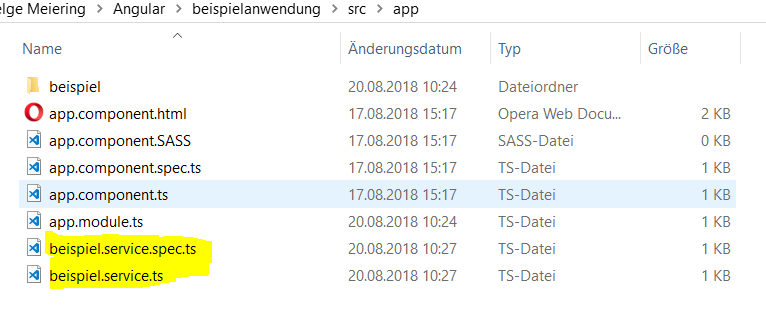
\includegraphics[scale=0.9]{content/pictures/services.png}
	% bosch_iot_poll.png: 0x0 pixel, 300dpi, 0.00x0.00 cm, bb=
	\caption{ Dateien eines Services}
	\label{fig:service}
\end{figure}

\subsection{Direktiven}
Direktiven können eine Ansicht verändern oder mehr Informationen weitergeben. Es wurden keine Direktiven in dieser Arbeit selbst entwickelt, jedoch sind sie ein wichtiger Teil, da viele Fremddirektiven zum Einsatz kamen. Direktiven werden in zwei Gruppen geteilt. Zum einen haben wir die Attibutsdirektiven. Dazu gehören auch die selbst Geschrieben Components. Sie heißen Attributsdirektiven, weil Sie wie ein Attribut einem \ac{HTML}-Tag mitgegeben werden. Ein Beispiel hierfür ist das ngClass. Es kann durch den Programmcode die Klasse eines Tags verändern. Eine sehr häufig genutzte Direktive ist die Strukturdirektive. Sie Verändert die Struktur des \ac{HTML}-Codes. Strukturdirektiven erkennt man an dem vorangestellten *. So ist es möglich mit *ngFor ganze Arrays direkt im \ac{HTML}-Code auszugeben oder mit *ngIf \ac{HTML}-Code zu entfernen und nicht nur auszublenden. \autocite{Clow.2018}

\begin{lstlisting}[language=sh, frame=single]
$  ng genarate directive Beispiel
\end{lstlisting} 

\begin{lstlisting}[language=sh, frame=single]
$  ng g d Beispiel
\end{lstlisting}

Direktiven werden ebenfalls auf den fast gleichen Weg erstellt. Und der Name wäre in diesem Fall DirectivBeispiel. So können alle zusammengehörenden Bereiche den gleichen Namen haben und doch eine andere Aufgabe übernhemen.

\begin{figure}[H]
	\centering
	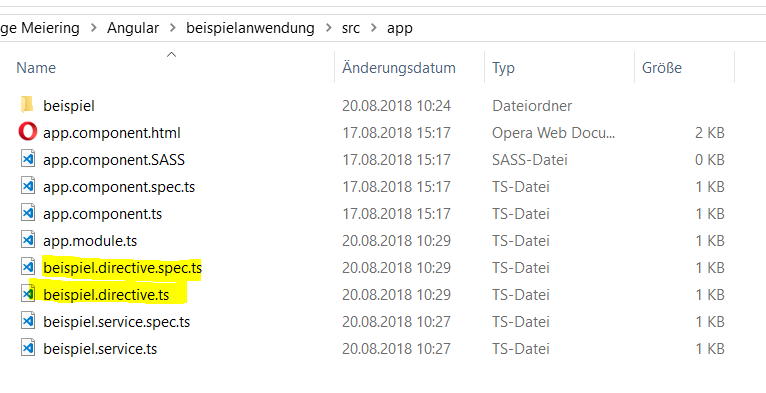
\includegraphics[scale=0.9]{content/pictures/directive.png}
	% bosch_iot_poll.png: 0x0 pixel, 300dpi, 0.00x0.00 cm, bb=
	\caption{ Dateien einer Direktiven}
	\label{fig:directive}
\end{figure}




\section{Backend}
Das Inventarsierungssystem kommt mit einem Fronent alleine nicht aus. Jedes größere Projekt teilt sich auch in ein Backend auf. Berechnungen, der Login und auch Netzwerkanfragen sind Dinge, die im Hintergrund der Anwendung geschehen. Der User soll von diesen dingen nichts mitbekommen. Für ihn müssen sie, wie selbstverständlich Funktionieren. In Kapitel \ref{chapter:frameworkchoice} wurde die Große vielfalt der Frameworks erwähnt. Es wurde auch kurz erläutert warum welches Framework gewählt wurde. In diesem Kapitel soll detaillierter in das Framework Laravel und seine Backendaufgaben geblickt werden.

\subsection{Laravel}
Mit \ac{PHP} existiert eine sehr mächtige Programmiersprache mit unzähligen Funktionen. Seit einigen Jahren ist \ac{PHP} objektorientierter. Dadurch fanden viele Entwickler schneller einen Zugang zu diesem mächtigen Werkzeug. Durch den riesen Umfang den \ac{PHP} nativ anbietet, leidet auch die Übersichtlichkeit. \ac{HTML} und \ac{PHP} kann sehr unübersichtlich vermischt werden, Datenbankabfragen sind häufig lange und kompliziert und das Entwickeln von einem LogIn-System kann viel Zeit in anspruch nehmen. Genau hier setzt das \ac{PHP} Framework Laravel ein. Mit seiner Renderengine Blade wird der vermischte Code übersichtlicher, die Datenbankabfragen werden kürzer und einfacher und ein LogIn-System ist schnell erstellt. Zusätzlich nutzt Laravel das bekannte \ac{MVC} Muster.\autocite{Laravel.2018}

\subsection{Installation von Laravel}
Wie für JavaScript, gibt es auch für \ac{PHP} einen Packagemanager. Dieser lädt Abhängigkeiten welche für Laravel nötig sind. Wie auch bei Angular, können hier Abhängikeiten nachinstalliert werden. Durch die große Community sind auch viele Erweiterungen frei zur Verfügung. Im ersten Schritt muss allerdings Composer installiert werden. Die Software steht kostenfrei auf \url{http://www.composer.com} zur Verfügung. Diese wird für Windows, Linux und MacOS angeboten. \autocite{Composer.2018} Unter Windows läuft die Installation über einen Assistenten. Ist eine \ac{PHP} Version welche neuer als 7.1.2 ist und die Extensions: OpenSSL, \ac{PDO}, Mbstring Tokenizer, \ac{XML}, Ctype und \ac{JSON} installiert, kann ein Laravel Projekt mit der Versionsnummer 5.6 sofort mit Composer angelegt werden und muss nicht wie Angular erst installiert werden.

\subsection{Artisan}

\subsection{Controller}

\subsection{REST}




\section{Security}

\subsection{CORS}

\subsection{Token}

\subsection{Salt}


\section{Deploy}

\subsection{Deploy in Angular}
\subsection{Deploy in Laravel}
